\documentclass{standalone}
\usepackage{tikz}
\usepackage{ctex,siunitx}
\setCJKmainfont{Noto Serif CJK SC}
\usepackage{tkz-euclide}
\usepackage{amsmath}
\usetikzlibrary{patterns, calc}
\usetikzlibrary {decorations.pathmorphing, decorations.pathreplacing, decorations.shapes,}

\begin{document}
\small
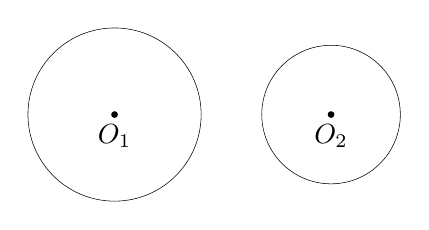
\begin{tikzpicture}[>=stealth,scale=1.1]
  \tkzSetUpPoint[fill=black]
  % \useasboundingbox(-1,-0.75)rectangle(3.7,1.4);
  \tkzDefPoints{0/0/O1,2.5/0/O2,0/1/A,2.5/0.8/B}
  \tkzDrawCircles[black](O1,A O2,B)
  \tkzDrawPoints(O1,O2)
  \tkzLabelPoint(O1){$O_1$}
  \tkzLabelPoint(O2){$O_2$}
\end{tikzpicture}
\end{document}